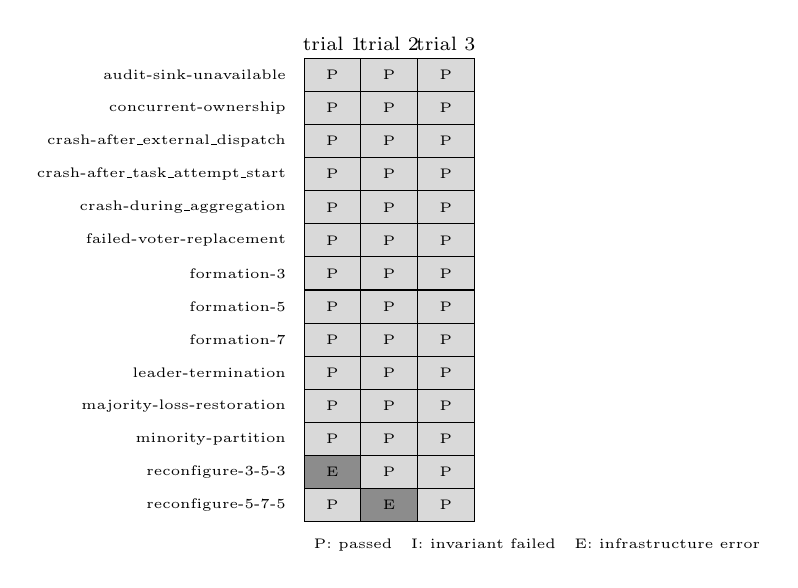
\begin{tikzpicture}[x=0.72cm,y=0.42cm]
\node[anchor=east,font=\tiny] at (-0.15,-0.5) {audit-sink-unavailable};
\draw[fill=black!15] (0,-1) rectangle (1,0);\node[text=black,font=\tiny] at (0.5,-0.5){P};
\draw[fill=black!15] (1,-1) rectangle (2,0);\node[text=black,font=\tiny] at (1.5,-0.5){P};
\draw[fill=black!15] (2,-1) rectangle (3,0);\node[text=black,font=\tiny] at (2.5,-0.5){P};
\node[anchor=east,font=\tiny] at (-0.15,-1.5) {concurrent-ownership};
\draw[fill=black!15] (0,-2) rectangle (1,-1);\node[text=black,font=\tiny] at (0.5,-1.5){P};
\draw[fill=black!15] (1,-2) rectangle (2,-1);\node[text=black,font=\tiny] at (1.5,-1.5){P};
\draw[fill=black!15] (2,-2) rectangle (3,-1);\node[text=black,font=\tiny] at (2.5,-1.5){P};
\node[anchor=east,font=\tiny] at (-0.15,-2.5) {crash-after\_external\_dispatch};
\draw[fill=black!15] (0,-3) rectangle (1,-2);\node[text=black,font=\tiny] at (0.5,-2.5){P};
\draw[fill=black!15] (1,-3) rectangle (2,-2);\node[text=black,font=\tiny] at (1.5,-2.5){P};
\draw[fill=black!15] (2,-3) rectangle (3,-2);\node[text=black,font=\tiny] at (2.5,-2.5){P};
\node[anchor=east,font=\tiny] at (-0.15,-3.5) {crash-after\_task\_attempt\_start};
\draw[fill=black!15] (0,-4) rectangle (1,-3);\node[text=black,font=\tiny] at (0.5,-3.5){P};
\draw[fill=black!15] (1,-4) rectangle (2,-3);\node[text=black,font=\tiny] at (1.5,-3.5){P};
\draw[fill=black!15] (2,-4) rectangle (3,-3);\node[text=black,font=\tiny] at (2.5,-3.5){P};
\node[anchor=east,font=\tiny] at (-0.15,-4.5) {crash-during\_aggregation};
\draw[fill=black!15] (0,-5) rectangle (1,-4);\node[text=black,font=\tiny] at (0.5,-4.5){P};
\draw[fill=black!15] (1,-5) rectangle (2,-4);\node[text=black,font=\tiny] at (1.5,-4.5){P};
\draw[fill=black!15] (2,-5) rectangle (3,-4);\node[text=black,font=\tiny] at (2.5,-4.5){P};
\node[anchor=east,font=\tiny] at (-0.15,-5.5) {failed-voter-replacement};
\draw[fill=black!15] (0,-6) rectangle (1,-5);\node[text=black,font=\tiny] at (0.5,-5.5){P};
\draw[fill=black!15] (1,-6) rectangle (2,-5);\node[text=black,font=\tiny] at (1.5,-5.5){P};
\draw[fill=black!15] (2,-6) rectangle (3,-5);\node[text=black,font=\tiny] at (2.5,-5.5){P};
\node[anchor=east,font=\tiny] at (-0.15,-6.5) {formation-3};
\draw[fill=black!15] (0,-7) rectangle (1,-6);\node[text=black,font=\tiny] at (0.5,-6.5){P};
\draw[fill=black!15] (1,-7) rectangle (2,-6);\node[text=black,font=\tiny] at (1.5,-6.5){P};
\draw[fill=black!15] (2,-7) rectangle (3,-6);\node[text=black,font=\tiny] at (2.5,-6.5){P};
\node[anchor=east,font=\tiny] at (-0.15,-7.5) {formation-5};
\draw[fill=black!15] (0,-8) rectangle (1,-7);\node[text=black,font=\tiny] at (0.5,-7.5){P};
\draw[fill=black!15] (1,-8) rectangle (2,-7);\node[text=black,font=\tiny] at (1.5,-7.5){P};
\draw[fill=black!15] (2,-8) rectangle (3,-7);\node[text=black,font=\tiny] at (2.5,-7.5){P};
\node[anchor=east,font=\tiny] at (-0.15,-8.5) {formation-7};
\draw[fill=black!15] (0,-9) rectangle (1,-8);\node[text=black,font=\tiny] at (0.5,-8.5){P};
\draw[fill=black!15] (1,-9) rectangle (2,-8);\node[text=black,font=\tiny] at (1.5,-8.5){P};
\draw[fill=black!15] (2,-9) rectangle (3,-8);\node[text=black,font=\tiny] at (2.5,-8.5){P};
\node[anchor=east,font=\tiny] at (-0.15,-9.5) {leader-termination};
\draw[fill=black!15] (0,-10) rectangle (1,-9);\node[text=black,font=\tiny] at (0.5,-9.5){P};
\draw[fill=black!15] (1,-10) rectangle (2,-9);\node[text=black,font=\tiny] at (1.5,-9.5){P};
\draw[fill=black!15] (2,-10) rectangle (3,-9);\node[text=black,font=\tiny] at (2.5,-9.5){P};
\node[anchor=east,font=\tiny] at (-0.15,-10.5) {majority-loss-restoration};
\draw[fill=black!15] (0,-11) rectangle (1,-10);\node[text=black,font=\tiny] at (0.5,-10.5){P};
\draw[fill=black!15] (1,-11) rectangle (2,-10);\node[text=black,font=\tiny] at (1.5,-10.5){P};
\draw[fill=black!15] (2,-11) rectangle (3,-10);\node[text=black,font=\tiny] at (2.5,-10.5){P};
\node[anchor=east,font=\tiny] at (-0.15,-11.5) {minority-partition};
\draw[fill=black!15] (0,-12) rectangle (1,-11);\node[text=black,font=\tiny] at (0.5,-11.5){P};
\draw[fill=black!15] (1,-12) rectangle (2,-11);\node[text=black,font=\tiny] at (1.5,-11.5){P};
\draw[fill=black!15] (2,-12) rectangle (3,-11);\node[text=black,font=\tiny] at (2.5,-11.5){P};
\node[anchor=east,font=\tiny] at (-0.15,-12.5) {reconfigure-3-5-3};
\draw[fill=black!45] (0,-13) rectangle (1,-12);\node[text=black,font=\tiny] at (0.5,-12.5){E};
\draw[fill=black!15] (1,-13) rectangle (2,-12);\node[text=black,font=\tiny] at (1.5,-12.5){P};
\draw[fill=black!15] (2,-13) rectangle (3,-12);\node[text=black,font=\tiny] at (2.5,-12.5){P};
\node[anchor=east,font=\tiny] at (-0.15,-13.5) {reconfigure-5-7-5};
\draw[fill=black!15] (0,-14) rectangle (1,-13);\node[text=black,font=\tiny] at (0.5,-13.5){P};
\draw[fill=black!45] (1,-14) rectangle (2,-13);\node[text=black,font=\tiny] at (1.5,-13.5){E};
\draw[fill=black!15] (2,-14) rectangle (3,-13);\node[text=black,font=\tiny] at (2.5,-13.5){P};
\node[font=\scriptsize] at (0.5,0.45) {trial 1};
\node[font=\scriptsize] at (1.5,0.45) {trial 2};
\node[font=\scriptsize] at (2.5,0.45) {trial 3};
\node[anchor=west,font=\tiny] at (0,-14.7) {P: passed\quad I: invariant failed\quad E: infrastructure error};
\end{tikzpicture}
